\documentclass[10pt,a4paper]{article}
\usepackage[textwidth=18cm,textheight=25cm]{geometry}
\usepackage[pdftex]{graphicx}
\usepackage{multirow}
% cv-custom.tex
%
% Custom macro commands and packages
% for formatting a Curriculum Vitae.
%
% Author: Matthew Earnshaw <matt@earnshaw.org.uk>
% Inspired by http://www.cv-templates.info/2009/03/professional-cv-latex/

\pagestyle{empty}

% Packages
\usepackage[usenames,dvipsnames]{color} % For custom colours
\usepackage{titlesec} % For custom section headings
\usepackage{mdwlist} % For compact lists
\usepackage[pdftex]{hyperref}
\usepackage{marvosym} % For icons

% Hyperlink colour and style
\definecolor{linkcolour}{rgb}{0,0.2,0.6}
\hypersetup{colorlinks,breaklinks, urlcolor=linkcolour, linkcolor=linkcolour}

% Custom colour
\definecolor{lgray}{gray}{0.4}

% Custom list bullet
\renewcommand{\labelitemi}{$\succ$}

% Header commands
\newcommand{\name}[1]{\LARGE\textbf{#1}}
\newcommand{\address}[1]{\color{lgray}{#1}}
\newcommand{\tel}[1]{\Large\Telefon~\small{#1}}
\newcommand{\email}[1]{\Large\Letter~\href{mailto:#1}{\small{#1}}}
\newcommand{\web}[2]{\Large\Mundus~\href{#1}{\small{#2}}}
	
% Section headings
\titleformat{\section}{\large\scshape\raggedright}{}{0em}{}[\titlerule]
\titlespacing{\section}{0pt}{0.6cm}{5pt}
% Note: Create an environment for sections ?

% Full width tables
\newenvironment{ftabular}[1]
{\begin{tabular*}{0.95\textwidth}{@{\extracolsep{\fill}}#1}}
{\end{tabular*}}

\usepackage[utf8]{inputenc}

\begin{document}
\footnotesize
\fontfamily{ptm}

\section{\sc K{\footnotesize İŞ\footnotesize İSEL} B{\footnotesize İLG\footnotesize İLER}}

\begin{tabular}{ l l l }
\vspace{0.5 mm}\\
\multirow{8}{*}{\fbox{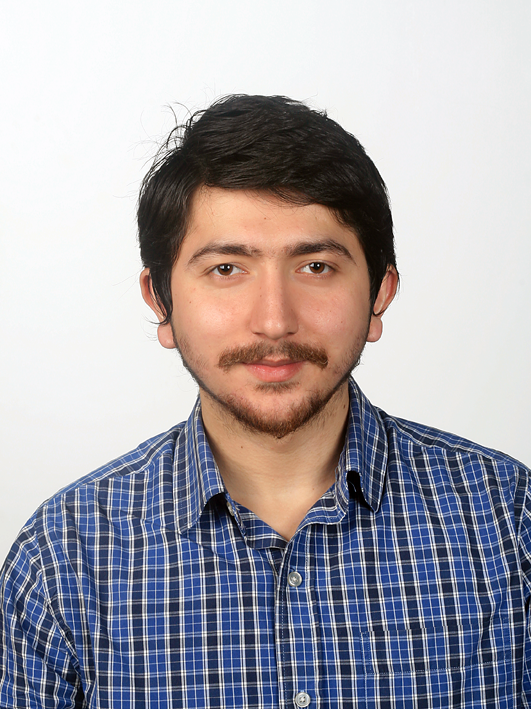
\includegraphics[height=25mm,width=20mm]{semih.png}}}
& {\Huge\name{Semih  Özköroğlu}}& Tarih: \small{08/07/2014}\\
\vspace{1 mm}\\
& \textbf{Adres :} \address{Atatürk Mah. 460. Sok. Hasbahçe Konakları Beylikdüzü/İSTANBUL} & \web{http://sozkoroglu.me}{semihozkoroglu.github.io}\\
& \textbf{Doğum Tarihi :} \address{18.11.1989} & \email{semihozkoroglu@gmail.com}\\
& \textbf{Medeni Hal :} \address{Bekar} & \tel{0506 3474727}\\
& \textbf{Askerlik Durumu  :} \address{Tecilli - Yüksek Lisans} & \web{http://www.linkedin.com/profile/view?id=181945022}{linkedin}\\
& \textbf{Engellilik Durumu :} \address{Yok} & \\
\end{tabular}

\section{\sc E{\footnotesize Ğ\footnotesize İT\footnotesize İM} B{\footnotesize İLG\footnotesize İLER\footnotesize İ}}
\hspace*{1.6in}\begin{tabular}{lr}
\vspace{0.5 mm}\\
\textbf{Eğitim Seviyesi :} & Üniversite / Yüksek Lisans \\
\vspace{0.5 mm}\\
\textbf{Üniversite :} & Sakarya Üniversitesi \\
\textbf{Fakülte/Enstitü :} & Fen Bilimleri Enstitüsü \\
\textbf{Bölüm :} & Bilişim Sistemleri \\
\textbf{Öğrenim Tipi / Dili :} & Örgün Öğretim / Türkçe\\
\textbf{Başlama / Mez. Tarihi :} & Şubat - 2014 / Okuyor\\
\vspace{0.5 mm}\\
\textbf{Üniversite :} & Samsun 19 Mayıs Üniversitesi \textbf{3.lük derecesi ile Mezun} \\
\textbf{Fakülte/Enstitü :} & Mühendislik Fakültesi \\
\textbf{Bölüm :} & Bilgisayar Mühendisliği \\
\textbf{Öğrenim Tipi / Dili :} & Örgün Öğretim / Türkçe\\
\textbf{Not Sist. / Mez. Derecesi :} & 100 / 77.31 \\
\textbf{Başlama / Mez. Tarihi :} & Eylül -2009 / Haziran -2012\\
\vspace{0.5 mm}\\
\textbf{Lise Türü / Bölüm :} & Düz Lise / Fen\\
\textbf{Öğrenim Tipi / Dili :} & Örgün Öğretim / Türkçe\\
\textbf{Lise Adı :} & izzet ünver\\
\textbf{Not Sist. / Mez. Derecesi :} & 100 / 83.50\\
\textbf{Başlama / Mez. Tarihi :} & Eylül - 2004 / Haziran-2007\\
\vspace{0.5 mm}\\
\end{tabular}

\section{\sc İ{\footnotesize Ş} D{\footnotesize ENEY\footnotesize İM\footnotesize İ}}
\begin{ftabular}{r|p{14cm}}
\textsc{Nisan-2013} & \textbf{Tmob - {\footnotesize İ}stanbul} \\
\vspace{0.5 mm}\\
 & \textbf{Pozisyon :} Android Geliştirici\\
 & \textbf{İşin Tanımı :} Denizbank, Atlasjet, Markafoni, Trendyol mobil uygulamalarının geliştirilmesi. Bug 'larının çözülmesi.\\

\multicolumn{2}{c}{ } \\ % Spacer 

\textsc{Aralık-2012 Nisan-2013} & \textbf{Tim Ticaret Net Bilişim - {\footnotesize İ}stanbul} \\
\vspace{0.5 mm}\\
 & \textbf{Pozisyon :} Android Geliştirici / Web Geliştirici\\
 & \textbf{İşin Tanımı :} Timplatform mobil uygulaması, web uygulamaları ve api servisleri geliştirilmesi.\\

\multicolumn{2}{c}{ } \\ % Spacer 

\textsc{Kasım–2011 Haziran-2012} & \textbf{Omü mühendislik fakültesi - Samsun} \\
\vspace{0.5 mm}\\
 & \textbf{Pozisyon :} Web Geliştirici / Sistem Yöneticisi\\
 & \textbf{İşin Tanımı :} Wordpress tabanlı mühendislik fakültesi web servisinin bakımı, güncellenmesi, tasarımı yapılmıştır.\\

\multicolumn{2}{c}{ } \\ % Spacer 

\textsc{Ekim-2010 Haziran-2011} & \textbf{Omü endüstri mühendisliği – Samsun} \\
\vspace{0.5 mm}\\
 & \textbf{Pozisyon :} Web Geliştiricisi\\
 & \textbf{İşin Tanımı :} Mühendislik fakültesi bölüm labratuvarlarının kurulumu. Web sitesilerinin geliştirilmesi\\

\multicolumn{2}{c}{ } \\ % Spacer 

\textsc{Temmuz-2011} & \textbf{Dsmart - {\footnotesize İ}stanbul (Stajyer)} \\
\vspace{0.5 mm}\\
 & \textbf{Pozisyon :} Sistem Gelişticisi\\
 & \textbf{İşin Tanımı :} Redmine sisteminin kurulumu, ldap bağlantısı ve özelleştirme çalışması\\

\end{ftabular}

\section{\sc P{\footnotesize ROJELER}}
\begin{ftabular}{r|p{15cm}}

\textsc{Android} & \textbf{DenizBank Tablet ve Phone} \\
  \vspace{0.5 mm}\\
& DenizBank mobil bankacılık uygulaması ile müşterilerine tüm bankacılık işlemlerini\\ 
& mobil uygulama üzerinden gerçekleştirmesini sağlamaktadır.\\
& \web{https://play.google.com/store/apps/details?id=com.tmob.tabletdeniz}{TabletDeniz} , \web{https://play.google.com/store/apps/details?id=com.tmob.denizbank}{PhoneDeniz}\\

\vspace{0.5 mm}\\
& \textbf{Nerede Ne Yenir} \\
  \vspace{0.5 mm}\\
& Kullanıcılar için bulundukları çevrede mekan önerisi ve mekan ile ilgili detaylı bilgi sahibi olmaları için\\ 
& geliştirilmekte olan sosyal bir uygulama. Bu uygulama sayesinde rezervasyon yapılması istenilen\\
& mekan ile önerilen yemekler veya içeçekler hakkında ve ulaşım hakkında detaylı bilgi sahibi olunmaktadır.\\

\vspace{0.5 mm}\\
& \textbf{Timplatform} \\
  \vspace{0.5 mm}\\
& Uygulamada kullanıcılar kendileri arasında mesajlaşabilmekte veya bir gruba mesaj gönderebilmektedir.\\ 
& Ayrıca timeline üzerinde kullanıcılar paylaşımda bulunabilmektedir.\\
& Bu paylaşımda resim gönderisinde de bulunabilmektedir.\\

 \vspace{0.5 mm}\\
& \textbf{Gmap} \\
  \vspace{0.5 mm}\\
& Uygulamaya giriş yapan kullanıcının lokasyon bilgisi alınmakta ve harita üzerinde işaretlenmektedir.\\
& Kullanıcı harita üzerinde gitmek istediği noktayı seçtiğinde, bulunduğu noktadan seçtiği noktaya gidebileceği\\
& yollar listelenmekte. Ve listelenen yollardan seçilen yol üzerinden hedef noktaya adım adım nasıl gidilebileceğini\\
& göstermektedir.\\

  \vspace{0.5 mm}\\
& \textbf{Barkod Okuyucu} \\
  \vspace{0.5 mm}\\
& Kameradan okunan barkod kodu ismiyle sd kart üzerinde klasör oluşturulması\\ 
& ve çekilen resimlerin bu klasöre kaydedilmesini sağlamaktadır.\\

\multicolumn{2}{c}{ } \\

\textsc{Django} &  Rest framework ile timplatform uygulaması için gerekli olan api servisinin gerçekleştirilmesi.\\
  \vspace{0.5 mm}\\
& İkmib Sektörel sitelerin gerçekleştirilmesi; \\ 
& \web{http://www.turkish-plastics.org/}{http://www.turkish-plastics.org/} \\
& \web{http://www.turkishconstruction.org/}{http://www.turkishconstruction.org/} \\
& \web{http://www.turkishhealthcare.org/}{http://www.turkishhealthcare.org/} \\
\multicolumn{2}{c}{ } \\

\textsc{Java Form} &  Yapay sinir ağları projesi gerçekleştirildi. Bu proje ile kullanıcıdan çift basamaklı sayıların çarpım tablosu alınmakta.\\ 
& Bu veriler ile algoritma eğitilmekte ve tek basamaklı sayıların çarpımları yaklaşık olarak belirlenen hata oranına göre\\ 
& hesaplanmaktadır. \\
& Kaynak: \web{https://github.com/semihozkoroglu/yapaysinir}{https://github.com/semihozkoroglu/yapaysinir} \\
\multicolumn{2}{c}{ } \\

\textsc{Python} & Kampuskart projesi. Bu projede smart card okuyucu ile haberleşerek mifare tipinde kartların üzerinde okuma, yazma işlemleri\\
& güvenlik maddelerinede dikkat edilerek gerçekleştirilmektedir. Bu projede kullanıcının kartına bakiye yükleme ve harcama\\
& noktalarında kartı ile alışveriş yapabilmesi prototip olarak tasarlanmış ve uygulanmıştır.\\
& Kaynak: \web{https://github.com/semihozkoroglu/kampuskart}{https://github.com/semihozkoroglu/kampuskart} \\
\multicolumn{2}{c}{ } \\

\vspace{0.5 mm}\\
\textsc{Matlab} & \textbf{Video İşleme} \\
\vspace{0.5 mm}\\
& Uygulamaya verilen video da kişilerin sarılma anı tespit edilmektedir.\\
& Kaynak: \web{https://github.com/semihozkoroglu/video-isleme}{https://github.com/semihozkoroglu/video-isleme} \\
& Youtube: \web{http://www.youtube.com/watch?v=OZWBbRdZWXI}{http://www.youtube.com/watch?v=OZWBbRdZWXI}\\

\vspace{0.5 mm}\\
& \textbf{Resim Sıkıştırma} \\
\vspace{0.5 mm}\\
& Jpeg algoritma standartı kullanılarak resim sıkıştırma işlemini gerçeleştirmektedir.\\
& Kaynak: \web{https://github.com/semihozkoroglu/Workspace/tree/master/compress}{https://github.com/semihozkoroglu/Workspace/tree/master/compress}\\

\multicolumn{2}{c}{ } \\

\end{ftabular}
\newpage

\hspace*{0.25in}\begin{ftabular}{r|p{25cm}}

\textsc{Rails} & Kampust Kart projesinde kullanıcıların kart bakiyesini ve kartı kullanım raporuna ulaşabilecekleri web arayüzü sunmaktadır.\\
& Kaynak: \web{https://github.com/semihozkoroglu/webproje}{https://github.com/semihozkoroglu/webproje}\\
\multicolumn{2}{c}{ } \\

\textsc{Javascript} & Google Javascript Map api kullanılarak gerçekleştirilmiştir. Projede tarayıcı üzerinden lokasyon bilgisi alınmakta\\
& ve kullanıcının bulunduğu noktadan gitmek istediği noktaya yol tarifi verilmektedir.\\
& Uygulama: \web{http://mes.pagodabox.com/app.html}{http://mes.pagodabox.com/app.html}\\
\vspace{0.5 mm}\\
& Places api sayesinde kullanıcının konumuna yakın olan yerlere erişilmektedir.\\
& Uygulama: \web{http://mes.pagodabox.com/interest.html}{http://mes.pagodabox.com/interest.html}\\
 
\multicolumn{2}{c}{ } \\

\textsc{C$ \# $} & Barkod oluşturma ve barkodlu ürün takip sistemi\\
& Kaynak: \web{https://github.com/semihozkoroglu/bedix}{https://github.com/semihozkoroglu/bedix}\\
\multicolumn{2}{c}{ } \\

\textsc{Bash} &  Bash scripting ile database temel düzeyde database uygulaması\\
& Kaynak: \web{https://github.com/semihozkoroglu/bash-database}{https://github.com/semihozkoroglu/bash-database} \\
\multicolumn{2}{c}{ } \\

\textsc{\LaTeX} & Cv şablonumu üretmek için yazdığım betik\\
& Kaynak: \web{https://github.com/semihozkoroglu/cv-creator}{https://github.com/semihozkoroglu/cv-creator}\\
\multicolumn{2}{c}{ } \\

\end{ftabular}
\section{\sc P{\footnotesize ROGRAMLAMA} B{\footnotesize İLG\footnotesize İS\footnotesize İ}}

{\bf Çok iyi}\\
\hspace*{0.3in}\begin{tabular}{lrrrrr}
\vspace{0.5 mm}\\
  $\bullet$ C &$\bullet$ Bash &$\bullet$ Java &$\bullet$ Python &$\bullet$ Matlab &\\
\end{tabular}
\vspace{0.5 mm}\\

{\bf Güzel}\\
\hspace*{0.3in}\begin{tabular}{lrrrr}
\vspace{0.5 mm}\\
  $\bullet$ C$ \# $ &$\bullet$ Ruby &$\bullet$ Rails & $\bullet$ Php & $\bullet$ Javascript\\
\end{tabular}
\vspace{0.5 mm}\\

{\bf Orta}\\
\hspace*{0.3in}\begin{tabular}{lrrrr}
\vspace{0.5 mm}\\
  $\bullet$ Qt Creator  & & & &\\
\end{tabular}
\vspace{0.5 mm}\\

{\bf İşletim sistemleri}\\
\hspace*{0.3in}\begin{tabular}{lrrrr}
\vspace{0.5 mm}\\
  $\bullet$ GNU/Linux ( iyi ) &$\bullet$ Windows\textregistered & & &\\
\vspace{0.5 mm}\\
\end{tabular}


{\bf Belgeleme uygulamaları}\\
\hspace*{0.3in}\begin{tabular}{lrrrr}
\vspace{0.5 mm}\\
  $\bullet$ \LaTeX & & & &\\
\end{tabular}
\vspace{0.5 mm}\\


\section{\sc K{\footnotesize URS }{\footnotesize ve }S{\footnotesize EM{\footnotesize İ}NERLER}}
\begin{ftabular}{r|p{14cm}}

\textsc{30-31 mart 2013} & \textbf{JsPyConf} \\
\vspace{0.5 mm}\\
 & \textbf{Kurum Adı :}  Özyeğin Üniversitesi\\

\multicolumn{2}{c}{ } \\

\textsc{8-10 mayıs 2012} & \textbf{Yeteneğe Destek Yaratıcı Ekonomiye Destek} \\
\vspace{0.5 mm}\\
 & \textbf{Kurum Adı :}  TTNET\\

\multicolumn{2}{c}{ } \\

\textsc{25-26-27 şubat 2011} & \textbf{Bilmök 7} \\
\vspace{0.5 mm}\\
 & \textbf{Kurum Adı :}  Yeditepe Üniversitesi\\
 
\multicolumn{2}{c}{ } \\

\textsc{2-3 nisan 2010} & \textbf{Özgür Yazılım Şenliği} \\
\vspace{0.5 mm}\\
 & \textbf{Kurum Adı :}  Bilgi Üniversitesi\\

\multicolumn{2}{c}{ } \\

\textsc{26-28 şubat 2009} & \textbf{ Bilmök 6 } \\
\vspace{0.5 mm}\\
 & \textbf{Kurum Adı :}  Selçuk Üniversitesi\\

\end{ftabular}

\section{\sc R{\footnotesize EFERANSLAR}}

\begin{tabular}{ l l l }
\vspace{1 mm}\\
\address{Ondokuz Mayıs Üniversitesi Yrd. Doç.} & \textbf{Recai Oktaş}& \email{roktas@bil.omu.edu.tr}\\
\vspace{1 mm}\\
\address{MetGlobal Django Developer} & \textbf{Zekeriya Koç}& \email{zekzekus@gmail.com}\\
\end{tabular}

\end{document}
